\chapter{BMA Posterior Distributions}\label{appendix}
\fixchapterheading

\vspace{0.7cm}

I will start with describing some of the characteristics of the Utah corrections system, such as the incarceration rate, cost per prisoner per day, etc., and maybe briefly mention how these compare with the U.S.  Using the results from the statistical analysis, the costs and benefits of certain types of corrections policy are considered.  It will be argued that certain policies, such as ignoring the employment needs of offenders, requiring them to pay restitution, etc., are unsound from an economic point of view.

Chapters 13 and 14 together serve as a survey of international
macroeconomics from W.W. II to the early 1980s.  This chapter
focuses to a greater degree on the Keynesian approach with its
emphasis on trade in goods and services, the current account
balance, multiplier effects, and policy within this context. Chapter
14 will focus on the more recent developments such as the greater
emphasis on asset markets in determining the exchange rate and the
monetary approach to the balance of payments.

This chapter provides a background to the proceeding chapters.
Issues that were of importance in the 1950s and 1960s shaped the
development of the discipline, so it is useful to study the history
of international macroeconomics in order to understand the
motivations behind current research in the field. There are three
main points that Kenen hopes to develop in the course of this
chapter: 

\begin{figure}[t]
\begin{center}
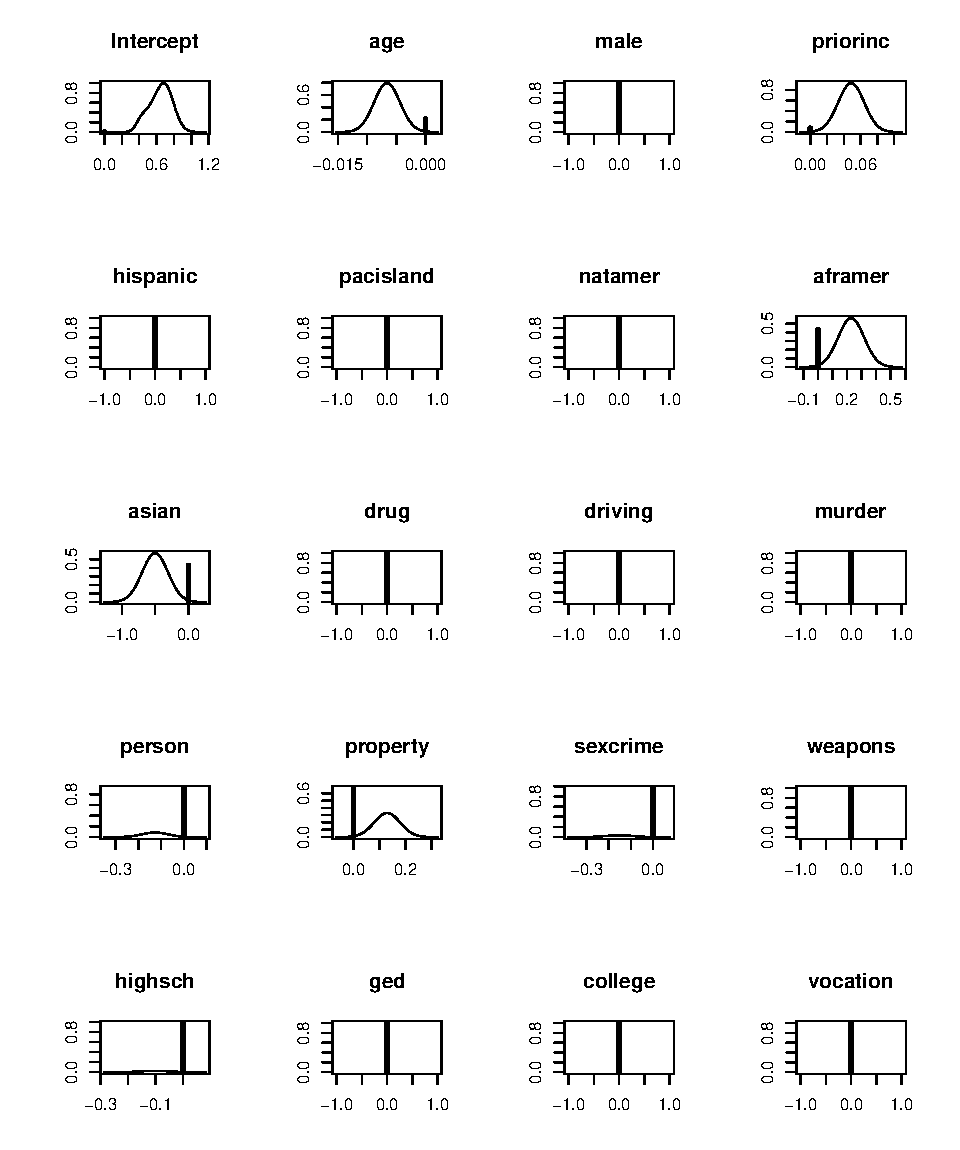
\includegraphics[height=20cm,width=14.5cm]{graphapp031.eps}
\caption{Posterior Distributions for Variables 1-19}
\end{center}
\end{figure}

Chapters 13 and 14 together serve as a survey of international
macroeconomics from W.W. II to the early 1980s.  This chapter
focuses to a greater degree on the Keynesian approach with its
emphasis on trade in goods and services, the current account
balance, multiplier effects, and policy within this context. Chapter
14 will focus on the more recent developments such as the greater
emphasis on asset markets in determining the exchange rate and the
monetary approach to the balance of payments.

This chapter provides a background to the proceeding chapters.
Issues that were of importance in the 1950s and 1960s shaped the
development of the discipline, so it is useful to study the history
of international macroeconomics in order to understand the
motivations behind current research in the field. There are three
main points that Kenen hopes to develop in the course of this
chapter: 

\begin{figure}[t]
\begin{center}
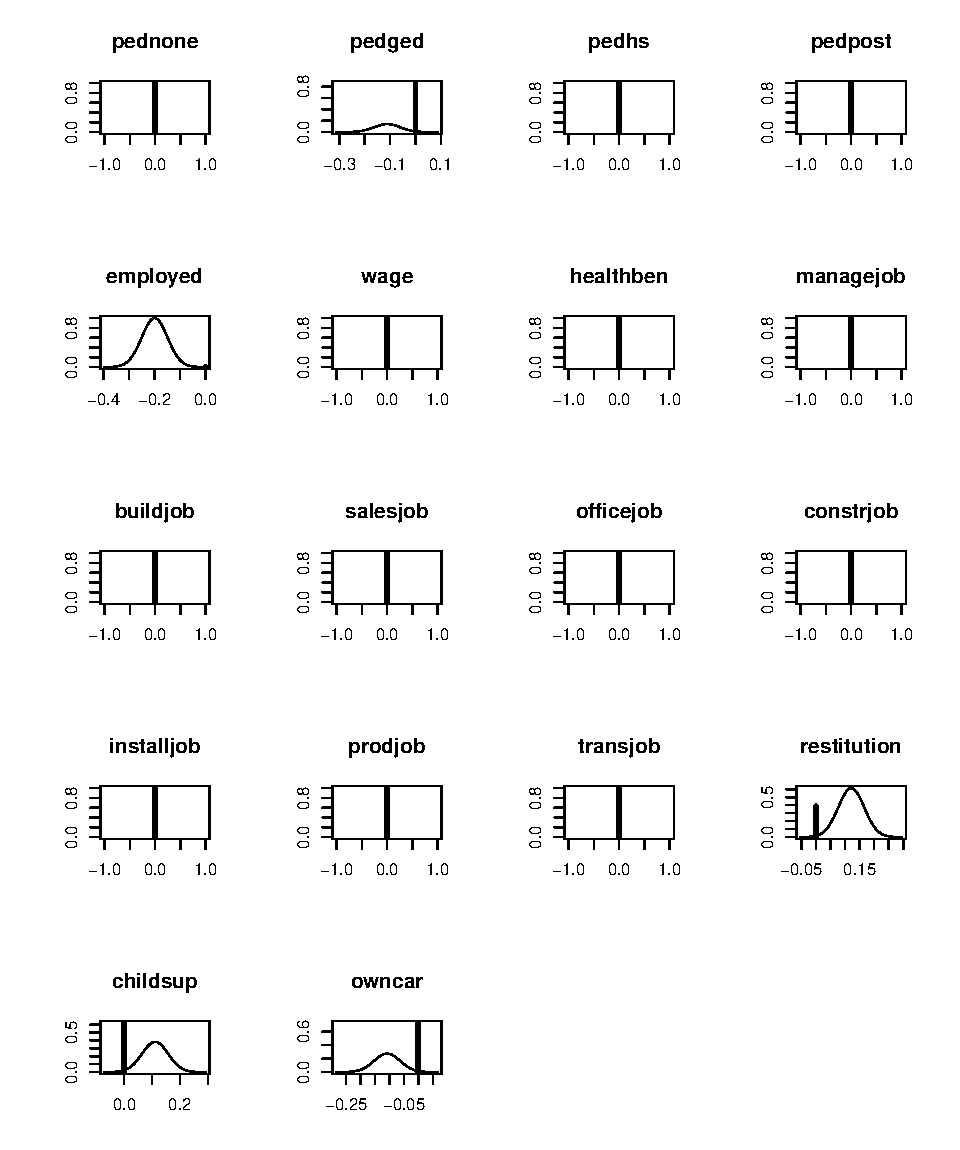
\includegraphics[height=20cm,width=14.5cm]{graphapp032.eps}
\caption{Posterior Distributions for Variables 20-37}
\end{center}
\end{figure}

Chapters 13 and 14 together serve as a survey of international
macroeconomics from W.W. II to the early 1980s.  This chapter
focuses to a greater degree on the Keynesian approach with its
emphasis on trade in goods and services, the current account
balance, multiplier effects, and policy within this context. Chapter
14 will focus on the more recent developments such as the greater
emphasis on asset markets in determining the exchange rate and the
monetary approach to the balance of payments.

This chapter provides a background to the proceeding chapters.
Issues that were of importance in the 1950s and 1960s shaped the
development of the discipline, so it is useful to study the history
of international macroeconomics in order to understand the
motivations behind current research in the field. There are three
main points that Kenen hopes to develop in the course of this
chapter: 

%\begin{figure}[t]
%\begin{center}
%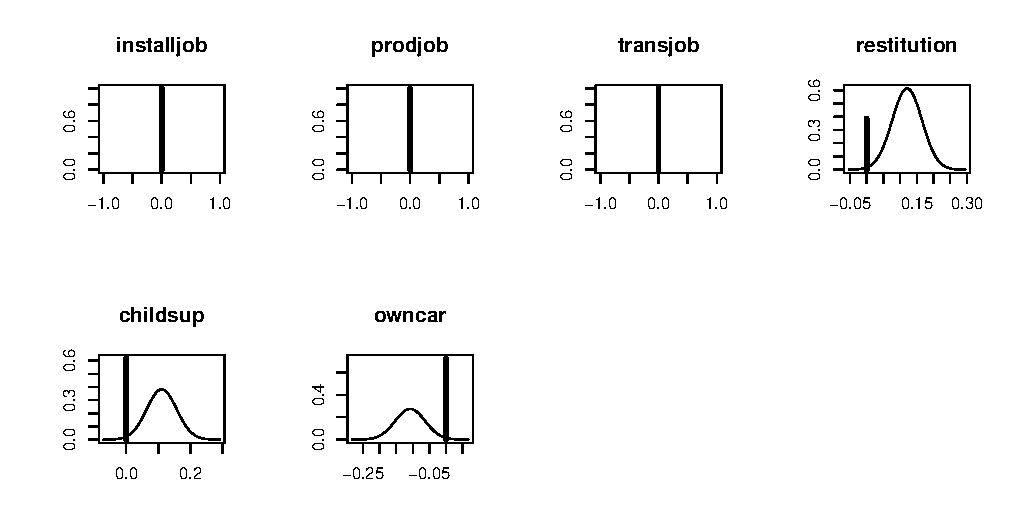
\includegraphics[clip=true,viewport=0mm 0mm 168mm 180mm, scale=0.85]{graphapp013.eps}
%\caption{Posterior Distributions for Variable 32-37}
%\end{center}
%\end{figure}
